% report_31_01_2018.tex
% Omkar H. Ramachandran
% omkar.ramachandran@colorado.edu
%
% Documentation for hemispheric dependence in the Fermi Pass 8 data
%

\documentclass[english]{article}
\usepackage[T1]{fontenc}
\usepackage[latin9]{inputenc}
\usepackage{geometry}
\geometry{verbose,tmargin=1.5in,bmargin=1.5in,lmargin=1.5in,rmargin=1.5in}
\usepackage{babel}
\newcommand{\GeV}{\,{\rm GeV}}
\newcommand{\MHz}{\,{\rm MHz}}
\usepackage{graphicx}
\graphicspath{{./plots/}}
\usepackage{hyperref}
\usepackage{listings}
\usepackage{color}

\lstdefinestyle{custompy}{
  belowcaptionskip=1\baselineskip,
  breaklines=true,
  frame=L,
  xleftmargin=\parindent,
  language=Python,
  showstringspaces=false,
  basicstyle=\footnotesize\ttfamily,
  keywordstyle=\bfseries\color{green},
  commentstyle=\itshape\color{red},
  identifierstyle=\color{black},
  stringstyle=\color{blue},
}

\lstset{escapechar=@,style=custompy}

\begin{document}
\title{Prelab 4 : Op-Amps 1}
\author{Omkar H. Ramachandran}

\maketitle

Note: I do not have Mathematica installed on my work laptop - which is an 8+ 
year old Lenovo flex 10. Thus, I have completed all the prelab activities in
Python and have written it up in \LaTeX. In addition, all the code present in
this document is available on my 
\href{https://github.com/ShadowWarden/electronics}{Github repository}

\section{Properties of an Op-Amp}
Using the TI documentation for the LF356 found \href{http://www.ti.com/lit/ds/symlink/lf356.pdf}{here},
we note the following characteristic values for the Op-Amp. I am only listing
the typical values for the device:
\begin{itemize}
	\item $f_T = 5\ \MHz$
	\item $A_0 = 200\ V/mV = 2\times10^{5}$
	\item $V_0 = \pm 13\ V$
	\item $I_{max} = 7\ mA$
	\item $R_i = 10^{12}\ \Omega$
\end{itemize}

\section{Non-Inverting Amplifier}
\subsection{Calculate gain given $R_f$ and $R$}
For a non-inverting amplifier, we know that the gain $G_0$ is as follows:
$$ G_0 = 1+ \frac{R_f}{R} $$
In our case, we have
\begin{itemize}
	\item $R_f = 10\ k\Omega$, $R = 100\ \Omega$. $G = 101.0$
	\item $R_f = 0$, $R = \infty$. $G = 1+0 = 1.0$
\end{itemize}
If we have $R_f = 10\ k\Omega$ and $R = 100\ \Omega$, given $V_{in}$, we can
compute $V_{out}$ as follows:
\begin{itemize}
	\item $V_{in}=1\ mV$. Thus, $V_{out} = GV_{in}\rightarrow V_{out} = 0.101\ V$
	\item $V_{in}=1\ V$. Then, $V_{out} = 13\ V$. In essence, the maximum voltage
		that the amplifier can provide is limited by the maximum power of the device.
		We know from our amplifier data that the maximum voltage it will allow is 
		$13\ V$
\end{itemize}
\subsection{Understanding device behavior}
\begin{figure}
	\centering
	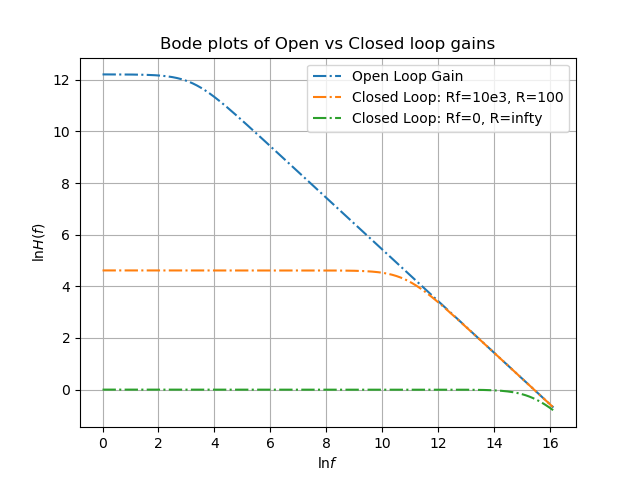
\includegraphics[scale=0.7]{bode_plots_overlaid.png}
	\caption{Overlaid Bode plots for the Open Loop Gain and the Two closed loop gains computed
	in the previous section}
	\label{fig:bode_overlaid}
\end{figure}

\subsubsection{Estimating input impedance}
Assume $R_f = 10\ k\Omega$, $R = 100\ \Omega$ and $f = 1\ kHz$. 
We know that the device's input impedance is as follows:
$$ R_i '=R_i(1+\frac{A_0}{1+j\frac{f}{f_0}}\frac{R}{R+R_f}) $$
$$ R_i' = \frac{R_i(R+R_f)\left(1+j\frac{f}{f_0}\right)+R_i A_0 R}{(R+R_f)\left(1+j\frac{f}{f_0}\right)}$$
We can attempt to estimate this impedance by computing the absolute value of $R_i'$.
Thus,
$$ \left|R_i'\right| = \frac{\left((R_i A_0 R+R_i(R+R_f))^{2}+\left(\frac{f}{f_0}R_i(R+R_f)\right)^{2}\right)^{1/2}}
						{\left((R+R_f)^{2}+\left[\frac{(R+R_f)f}{f_0}\right]^{2}\right)^{1/2}}
$$
Plugging in the values to \lstinline{input_Z()} function defined in \lstinline{lab4.py},
we obtain an input impedance of 
$$ Z = 3.148\times10^{16}\ \Omega $$

For the output impedance, we use $R_o = 40\ \Omega$. Thus, using the formula, we have
$$ R_o' = R_o/(1+AB)=R_o/(1+\frac{A_0}{1+j\frac{f}{f_0}}\frac{R}{R+R_f})$$
$$ R_o' = R_o/\left(1+\frac{A_0R}{\left(1+j\frac{f}{f_0}\right)(R+R_f)}\right) $$
Thus,
$$ R_o' = \frac{R_o(R+R_f)(1+j\frac{f}{f_0})}{(R+R_f)(1+j\frac{f}{f_0})+A_0R} $$
Once again, we estimate the impedance by measuring the absolute value of $R_o'$,
to get the following:
$$ \left|R_o'\right| = \frac{\left((R_0(R+R_f))^{2}+(R_0(R+R_f)f/f_0)^{2}\right)^{0.5}}{\left((A_0R+R+R_f)^{2}+((R+R_f)f/f_0)^2\right)^{0.5}}$$
Plugging in relevant values to \lstinline{output_Z()} function in 
\lstinline{lab4.py}, we find that the output impedance for a 1 kHz signal is 
$$ Z_{out} = 0.8076\ \Omega$$

\section{Questions about the Lab}
\begin{itemize}
	\item Overall, it looks like Part 4b is going to be the hardest overall.
		The frequency dial on the function generator has a slight error which
		causes the measure cursor to be off a little bit. It may be that, in this
		case, we can make do with an error of $O(10\ Hz)$, which might make it
		easier
	\item What happens if the power rail can supply less power overall than the
		maximum gain of the Op-Amp? Does the output voltage stick to the maximum
		voltage of the Op-Amp or is it the maximum allowed voltage of the rail?
\end{itemize}

\end{document}
